\documentclass[a4paper,10pt]{scrartcl}
\usepackage[utf8]{inputenc}
\usepackage{amsmath}
\usepackage[pdftex]{graphicx}
%\usepackage{algorithm}
%\usepackage{algpseudocode}
\usepackage{tikz}
\usepackage{float}
%opening
\title{CSC418 Assignment 2}
\author{Philip Lee - 9999074932}
\setlength{\parindent}{0cm}
\begin{document}

\maketitle

\section{Transformations}

\subsection{}

We are given three point mappings. An arbitrary affine 2D transformation has 6 unknowns. Thus we must solve for the following matrix $A$ with unknowns $a,b,c,d,e,f,$ that satisfies
the equation
\[ \begin{bmatrix}
      x_o \\ 
      y_o \\
      1
   \end{bmatrix} = A 
   \begin{bmatrix}
      x \\ 
      y \\
      1
   \end{bmatrix}
\]

\[A = \begin{bmatrix}
		  a & b & c \\
		  d & e & f \\
		  0 & 0 & 1
    \end{bmatrix}\]
    
The three point mappings are as follows: $(2,3) \rightarrow (10,8), (1,2) \rightarrow (8,-4), \\(3,-1) \rightarrow (2,0)$ 

From the matrix, we have the equations $x_o = ax + by + c, y_o = dx + ey + f$. Substituting in the points, we get the following system of equations written in matrix form:

% \begin{align} 10 &= 2a + b3 + c \\
%     8 &= 2d + e3 + f \\
%     9 &= a + 2b + c \\
%     -4 &= d + 2e + f \\
%     2 &= 3a - b + c \\
%     0 &= 3d - e + f \\
% \end{align}

\[ \begin{bmatrix}
      10 & 8 & 2 \\
      8 & -4 & 0 \\
      1 & 1 & 1\\
   \end{bmatrix} = AX,
   \hspace{1cm}X = \begin{bmatrix}
      2 & 1 & 3\\
      3 & 2 & -1\\
      1 & 1 & 1
   \end{bmatrix}
\]

Solving this equation gives

\[ X^{-1} = 
  \begin{bmatrix}
      0.6 & 0.4 & -1.4\\
      -0.8 & -0.2 & 2.2\\
      0.2 & -0.2 & 0.2
   \end{bmatrix}\]
   
and

\[
  A =   \begin{bmatrix}
      0 & 2 & 4\\
      8 & 4 & -20\\
      0 & 0 & 1
   \end{bmatrix}\], which is the affine transformation that maps the specified triangle.
   
\subsection{}

A general 2D homography has 8 unknowns. Thus {\bfseries four} point mappings are required to fully specify it.\\

A rigid 2D transform preserves lengths of lines and angles, including translation and rotation. The parameters are rotation angle $\theta$ and $t_x, t_y$. Thus {\bfseries two} point mappings
are required to uniquely determine this transformation.


\subsection{}
\subsubsection{Centroid}
The centroid of three points is preserved after projection. Consider the points $p_o(x_o, y_o, z_o), p_1(x_1, y_1, z_1)$ and $p_2(x_2, y_2, z_2)$. 

Consider 2 cases: 
\begin{enumerate}
 \item Find the centroid in 3D space then project onto 2D space
 \item Project all 3D points to 2D space then find the centroid
\end{enumerate}

{\bfseries Case 1}

The centroid in 3D space is 
\[ \begin{bmatrix}
    \frac{x_o + x_1 + x_2}{3}\\
    \frac{y_o + y_1 + y_2}{3}\\
    \frac{z_o + z_1 + z_2}{3}\\
  \end{bmatrix}
\]

After an affine projection, the z coordinate is discarded, which results in the centroid being
\[\begin{bmatrix}
    \frac{x_o + x_1 + x_2}{3}\\
    \frac{y_o + y_1 + y_2}{3}\\
  \end{bmatrix}\]

{\bfseries Case 2}

When all points are projected to 2D space, the result is $p_{op} = (x_o, y_o) , p_{1p} = (x_1, y_1), p_{2p} = (x_2, y_2)$

The centroid of these points is \[\begin{bmatrix}
    \frac{x_o + x_1 + x_2}{3}\\
    \frac{y_o + y_1 + y_2}{3}\\
  \end{bmatrix}\]
  
which is the same as in Case 1. Thus the centroid is preserved.


\subsubsection{Orthocenter}
The orthocenter of three points is not preserved after projection. Consider the points $p_o = (1, 1, 4), p_1 = (-1, 1, 4)$ and $p_2 = (0, 0, 5)$.\\

\pagebreak
{\bfseries Case 1}

The orthocenter in is calculated as follows. Find the line $l_o$ that joins $p_o$ and $p_1$, then find the line normal
to $l_o$ that intersects $p_2$. Do the same for $l_1$ that joins $p_1$ and $p_2$ and find the intersection to 
determine the orthocenter.

\[ l_o = \begin{bmatrix}
          0 \\
          1 \\
          4 \\
         \end{bmatrix} + t
         \begin{bmatrix}
          1 \\
          0 \\
          0 \\
         \end{bmatrix} \hspace{2cm}
  l_1 = \begin{bmatrix}
	    -1 \\
	    1 \\
	    4 \\
	  \end{bmatrix} + t
	  \begin{bmatrix}
	    1 \\
	    -1 \\
	    1 \\
	  \end{bmatrix}
\]

The line passing through $p_2 = (0, 0, 5)$ and intersects with $l_1$ is

\[
  n_o = \begin{bmatrix}
          0 \\
          0 \\
          5 \\
         \end{bmatrix} + u_o
         \begin{bmatrix}
          0 \\
          1 \\
          -1 \\
         \end{bmatrix} \hspace{2cm}
\] and intersects $l_o$ at $u_o = 1$

Similarly, the line passing through $p_1 = (1, 1, 4)$ and intersects/is normal with $l_1$ is

\[
  n_1 = \begin{bmatrix}
          1 \\
          1 \\
          1 \\
         \end{bmatrix} + u_1
         \begin{bmatrix}
          -4 \\
          -2 \\
          2 \\
         \end{bmatrix} \hspace{2cm}
\]

The intersect and therefore orthocenter of the triangle in 3D space is at $u_o = 0.5$ and $u_1 = 0.25$
at point $(0, 0.5, 4.5)$.\\

After projection, the orthocenter is $(0, 0.5)$\\

{\bfseries Case 2}

After projection from 3D to 2D, the points are $p_o = (1, 1), p_1 = (-1, 1)$ and $p_2 = (0, 0)$.\\

This is a right angled triangle. The orthocenter of a right angled triangle is a vertex, and in this case is $p_2 = (0,0)$

Since $(0, 0.5) \ne (0, 0)$ the orthocenters do not match, thus they are not preserved after projection.


\section{Cameras}

\subsection{}

The lens in a real camera serves to focus incoming light rays. Because the lens is able to focus
all parallel incoming rays, the brightness of the image is improved over that of a regular pinhole camera.
Increasing the aperture size increases the amount of light coming through but causes features to appear more blurry.
The focal length determines the distance from the lens that rays converge. The focal length determines
the angle of view and the magnification of the image. A shorter focal length reduces the magnification but
increases the field of view. A longer focal length improves magnification but reduces field of view.

\subsection{}

Given: $p_{eye} = (2, 1, 3)$, look-at point $p_{ref} = (-1, 2, 1)$ and up vector $v_{up} = (0, 1, 0)$

To determine the camera matrix, we require three basis vectors. The first vector $\vec w$ is obtained
as: 

\[ \vec w = p_{eye} - p_{ref}\]
\[ \vec w = (3, -1, 2)\]

Normalize $\vec w $
\[ \vec w_n = (3, -1, 2)/\sqrt{14}\]

Determine $\vec u = \vec w_n \times \vec v_{up}$ and normalize it

\[ \vec u = \begin{vmatrix} \vec i &\vec j &\vec k \\
	      3 & -1 & 2 \\
	      0 & 1 & 0\\             
            \end{vmatrix} = (-2, 0, 3)
\]

\[ \vec u_n = (-2, 0, 3) / \sqrt{13}\]

Determine $\vec v = \vec u \times \vec w$

\[ \vec v = \begin{vmatrix} \vec i &\vec j &\vec k \\
	      -2 & 0 & 3\\             
	      3 & -1 & 2 \\	      
            \end{vmatrix} = (-3, -13, -2)\]
            
\[ \vec v_n = (-3, -13, -2) / \sqrt{182}\]


So the camera matrix is:

\[ M_{CW} = \begin{bmatrix}
	      (\vec u_n) & (\vec v_n) & (\vec w_n) & (p_{ref}) \\
	      0 & 0 & 0 & 1
            \end{bmatrix} = 
            \begin{bmatrix}
	      -2/\sqrt{13} & -3/\sqrt{182} & 3/\sqrt{14} & 2 \\\
	      0 & -13/\sqrt{182} & -1/\sqrt{14} & 1 \\
	      3/\sqrt{13} & -2/\sqrt{182} & 2/\sqrt{14} & 3 \\
	      0 & 0 & 0 & 1\\
            \end{bmatrix}            
\]

The world to camera matrix is $M_{WC} = M_{CW}^-1$

\[ M_{WC} =    \begin{bmatrix}
	      -0.5547 & 0 & 0.8321 & -1.3 \\\
	      -0.22 & -0.963 & -0.14 & 1.85 \\
	      0.802 & -0.2673 & 0.53 & -2.94 \\
	      0 & 0 & 0 & 1\\
            \end{bmatrix}\]

\subsection{}            

Affine projection from 3D to 2D is given by \[A = \begin{bmatrix} 1 & 0 & 0 & 0 \\ 0 & 1 & 0 & 0 \\ 0 & 0 & 0 & 1 \end{bmatrix}\]

Points in the positive z direction must map to the plane $z = d$ because the view direction is $(0, 0, 1)$ and the image plane is at distance $d$ from the eye.
Using similar triangles an homogenous coordinates, this matrix is

\[ B =\begin{bmatrix}1 & 0 & 0 & 0\\
    0 & 1 & 0 & 0 \\
    0 & 0 & 1 & 0 \\
    0 & 0 & \frac{1}{d} & 0 \\
\end{bmatrix}\]
            
The product of these two matrices gives the projection matrix \[ P = AB = \begin{bmatrix} 1 & 0 & 0 & 0 \\ 0 & 1 & 0 & 0 \\ 0 & 0 & 1/d & 0 \end{bmatrix}\] 

Thus the 2D point is \[ \begin{bmatrix} x \\ y \\ 1\end{bmatrix} = P \begin{bmatrix} x_o \\ y_o \\ z_o \\ 1\end{bmatrix} = \begin{bmatrix} x_o \\ y_o \\ z_o/d\end{bmatrix} = \begin{bmatrix}x_od/z_o \\ y_od/z_o \\ 1\end{bmatrix}\]


\subsection{}

In general, parallel lines in the world do not remain parallel after they are projected to camera C. The only
case in which they would remain parallel after being projected is if the lines are perpendicular to the viewing
direction. \\

Consider the line $l$ with direction vector $\vec b = (b_x, b_y, b_z)$. Then any point on the line can be represented as
\[ P_o = P_{xyz} + t\vec b\] where $P_{xyz}$ is a point that lies on the line $l$. If the matrix $P$ which represents
camera $C$ is applied to $P_o$:

\[ P = \begin{bmatrix} 1 & 0 & 0 & 0 \\ 0 & 1 & 0 & 0 \\ 0 & 0 & 1/d & 0 \end{bmatrix}\]

Every point on the line in 3D space gets mapped to $P_o\,projected$:

\[ P_{o\,projected} = \begin{bmatrix} P_x + tb_x\\ P_y + tb_y\\ (P_z + tb_z)/d \end{bmatrix}= \begin{bmatrix}  d(P_x + tb_x)/(P_z + tb_z)\\ d(P_y + tb_y)/(P_z + tb_z)\\1 \end{bmatrix}\]

Now consider two lines $l_1$ and $l_2$. For the lines to be parallel in 3D world space, $\vec b = (b_x, b_y, b_z)$ 
must be the same for both $l_1$ and $l_2$. This means that $d, b_x, b_y, b_z$ are the same for $l_1$ and $l_2$, while
$P_x, P_y, P_z$ can be different.\\

What is the point of convergence as the line stretches to infinity in 3D space? If we assume $b_z$ to be positive, evaluate:
\[ \lim_{t \to \infty} P_{o\,projected} = \lim_{t \to \infty} \begin{bmatrix}  d(P_x + tb_x)/(P_z + tb_z)\\ d(P_y + tb_y)/(P_z + tb_z)\\1 \end{bmatrix} =
  \begin{bmatrix} db_x/b_z \\ db_y/b_z \\ 1\end{bmatrix}\]
  
Thus two parallel lines will converge at the point $(db_x/b_z, db_y/b_z)$ when projected from 3D space to 2D space. This point of convergence
does not depend on $P_x, P_y, P_z$. If $b_z = 0$ (the lines are perpendicular to the viewing axis), 
then the lines 'converge' at $(\infty, \infty)$, which indicates that they do not converge on 2D space.\\

{\bfseries Conclusion:}\\

Lines that are perpendicular to viewing axis do not converge when projected.\\
All other lines converge at $(db_x/b_z, db_y/b_z)$ upon being projected.




\section{Surfaces}

$f(x,y,z) = (R - \sqrt{(x^2 + y^2) \,})^2 + z^2 - r^2 = 0$, where $ R > r$

\subsection{Find surface normal}


Need to find \[ \vec n = \nabla f\]
\[ \nabla f = ( \frac{\partial f}{\partial x}, \frac{\partial f}{\partial y}, \frac{\partial f}{\partial z})\]
\[ \frac{\partial f}{\partial x} = \frac{\partial ((R - \sqrt{(x^2 + y^2) \,})^2 + z^2 - r^2)}{\partial x}\]

Let $u = \sqrt{x ^2 + y^2}$, $\frac{\partial u}{\partial x} = \frac{x}{\sqrt{x ^2 + y^2}}$

Do substitution of $u$ into $f$

\[ \frac{\partial f}{\partial x} = \frac{\partial (R - u)^2}{\partial u} * \frac{\partial u}{\partial x}\]
\[ = -2 (R - \sqrt{x^2 + y^2}) * \frac{x}{\sqrt{x^2 + y^2}}\]
\[ = 2x - \frac{2Rx}{\sqrt{x^2+y^2}}\]

Similarly, 
\[\frac{\partial f}{\partial y} = 2y - \frac{2Ry}{\sqrt{x^2+y^2}}\]

And

\[\frac{\partial f}{\partial z} = 2z\]

such that \[ \vec n = \nabla f = (2x - \frac{2Rx}{\sqrt{x^2+y^2}}, 2y - \frac{2Ry}{\sqrt{x^2+y^2}}, 2z)\]

% Finally,
% 
% \[|\nabla f| = \sqrt{\frac{\partial f}{\partial x}^2 + \frac{\partial f}{\partial y}^2 + \frac{\partial f}{\partial z}^2}\]
% 
% \[ = (2x - \frac{2Rx}{\sqrt{x^2+y^2}})^2 + (2y - \frac{2Ry}{\sqrt{x^2+y^2}})^2 + (2z)^2\]
% \[ = \]

\subsection{}

Given a point $p = (x_o, y_o, z_o)$ that lies on the torus, implicit equation for tangent plane at $p$ is found by evaluating
$\nabla f $ at $p$.

\[ \nabla f(p) = (a,b,c) = (2x_o - \frac{2Rx_o}{\sqrt{x_o^2+y_o^2}}, 2y_o - \frac{2Ry_o}{\sqrt{x_o^2+y_o^2}}, 2z_o) \]
\[ ax + by + cz + d = 0\]

Evaluate the implicit equation at $p$ with values of $a, b, c$ to determine the constant $d$.

\[ d = -( x_o (2x_o - \frac{2Rx_o}{\sqrt{x_o^2+y_o^2}}) + y_o (2y_o - \frac{2Ry_o}{\sqrt{x_o^2+y_o^2}}) + z_o(2 z_o) )\]
\[ a = (2x_o - \frac{2Rx_o}{\sqrt{x_o^2+y_o^2}})\]
\[ b = (2y_o - \frac{2Ry_o}{\sqrt{x_o^2+y_o^2}})\]
\[ c = 2z\]

Substitute values of $a,b,c, d$ to obtain the implicit equation of the tangent plane at $p$.

\[ (2x_o - \frac{2Rx_o}{\sqrt{x_o^2+y_o^2}})x + (2y_o - \frac{2Ry_o}{\sqrt{x_o^2+y_o^2}})y + (2z_o)z -( x_o (2x_o - \frac{2Rx_o}{\sqrt{x_o^2+y_o^2}}) + y_o (2y_o - \frac{2Ry_o}{\sqrt{x_o^2+y_o^2}}) + z_o(2 z_o) ) = 0\]

\subsection{}

\[ q(\lambda) = (R\cos\lambda, R\sin\lambda, r)\]

Substitute $q(\lambda)$ into equation of surface $f$.

\[f(R\cos\lambda, R\sin\lambda, r) = R - \sqrt{R^2\cos^2{\lambda} + R^2\sin^2{\lambda}\,} + r^2 - r^2 = 0\]
\[ = R - \sqrt{R^2(\cos^2{\lambda} + \sin^2{\lambda})} = 0\]

This satisfies the equation of the surface so $q(\lambda)$ lies on the torus.

\subsection{}

Tangent vector of $q(\lambda)$ is given by $ \frac{dq}{d\lambda} = (-R\sin\lambda, R\cos\lambda, 0) $

\subsection{}

The tangent vector of $q(\lambda)$ lies on the plane if the tangent vector is perpendicular to the plane's
normal and $q(\lambda)$ shares one point with the tangent plane. From 1.3, we already know that $q(\lambda)$ lies on
the surface of $f$ so there must already be a shared point. Check that the tangent vector is perpendicular to there
plane's normal at $p_q$, where $p_q$ has coordinates $x_o = R\cos\lambda, y_o = R\sin\lambda, z_o = r$

\[\nabla f(p_q) = (2R\cos\lambda - \frac{2R * 2R\cos\lambda}{\sqrt{4R^2\cos\lambda + 4R^2\sin\lambda}}, 2R\sin\lambda - \frac{2R * 2R\sin\lambda}{\sqrt{4R^2\cos\lambda + 4R^2\sin\lambda}}, 2r)\]
\[\nabla f(p_q) = (0, 0, 2r)\]

Check if the gradient at $p_q$ is perpendicular to tangent vector of $q(\lambda)$

\[q(\lambda) \bullet f(p_q) = (-R\sin\lambda, R\cos\lambda, 0) \bullet (0, 0, 2r) = 0\]

The dot product is $0$ so the tangent vector of $q(\lambda)$ and the normal of the tangent plane are perpendicular.

So therefore the tangent vector of $q(\lambda)$ lies on the tangent plane.


\section{}

\subsection{}
Some segments can be excluded from rendering by considering the viewing direction of the eye. If the
polygon is outside the eye's field of view, it can be excluded from rendering. This is a simple check that 
can be used to skip some segments of the BSP tree. \\

For example, if the viewing direction was along the outward normal of the $h$ polygon, then $b, g, i, e, c, d$ can be excluded
because they lie outside the eye's viewing volume.

\subsection{}

Below is the BSP tree for the planes. Some polygons ($c$ and $h$) were divided into multiple polygons.

\begin{figure}[H]
  \centering
  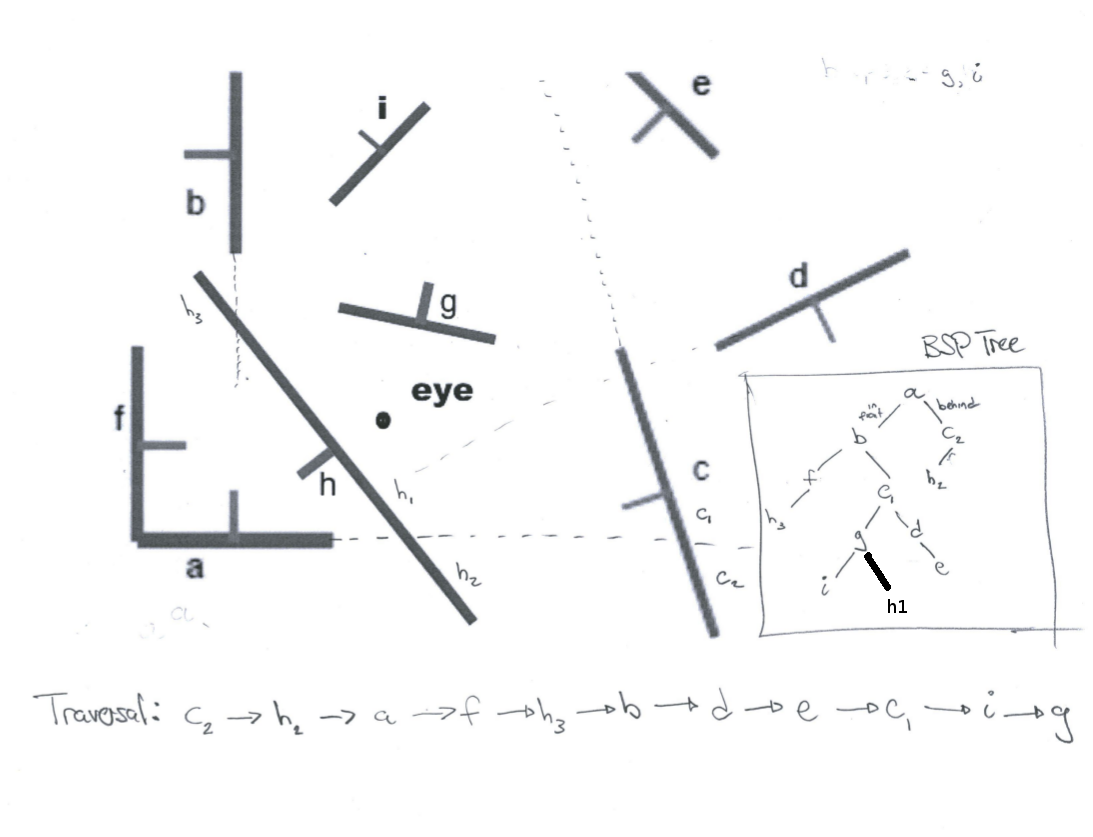
\includegraphics[trim = 2cm 4.5cm 1cm 0, clip, width=\linewidth, height=15cm]{q4.png}
\end{figure}




\subsection{}

The tree is traversed by following the algorithm:

Is the eye behind or in front of plane $X$? \\
If the eye is in front of plane $X$, draw everything behind $X$, then draw $X$, then draw everything in front of $X$\\
If the eye is behind plane $X$, draw everything in front of $X$, then draw $X$, then draw everything behind $X$ \\

Repeat until the entire tree is traversed. \\

This gives the following result:

$c_2 \to h_2 \to a \to f \to h_3 \to b \to d \to e \to c_1 \to i \to g \to h_1$



\end{document}
 